
\begin{figure}[htbp]
\renewcommand{\familydefault}{\sfdefault}\normalfont
\centering 
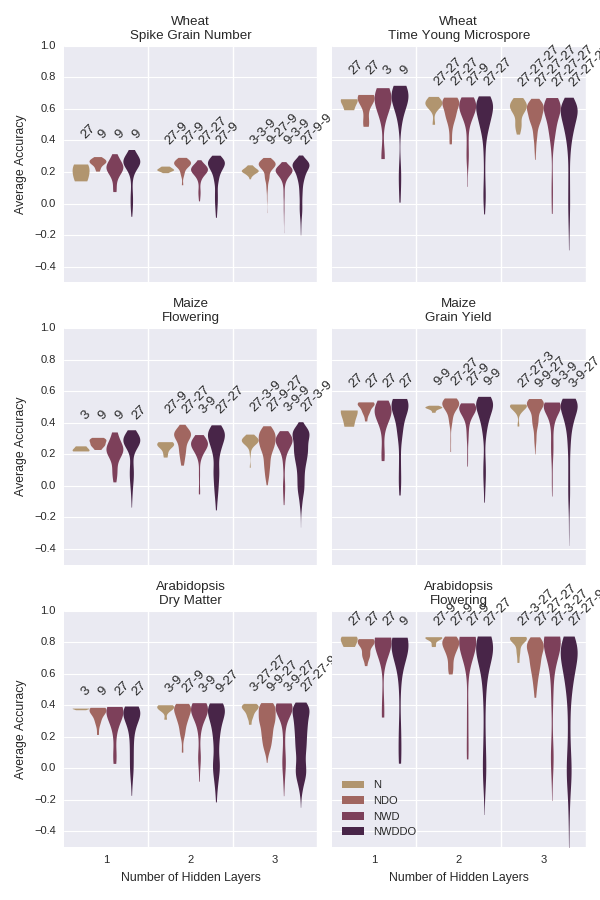
\includegraphics[keepaspectratio,height=\textheight,width=\linewidth]{g3_article/figures/depth_comparison.png}
    \caption{Distribution of predictive accuracy by benchmark dataset, network depth, 
             and model. The violin plot width indicates the Kernel Density Estimate 
             (KDE) of all observed accuraies of all models at a given network depth. 
             The sample size of the KDE is 7, 28, 28, and 112 samples for the 
             N, NWD, NDO, and NWDDO models, respectively. The models contributing 
             to each KDE vary across one or more of five weight decay, five dropout, 
             and seven hidden layer archetecture parameters and can be 
             understood as the distribution of results across the set of 
             hyper-parameters to all network models with the same depth and regularization
             type. The KDE bandwidth parameters are set using Scott's normal reference rule. 
             Negative accuraies are the result of trained models producing predictions that 
             are negatively correlated with actual measurements. The KDE plots are 
             trucated to the minimum and maximum observed prediction accuracies.} 
\label{fig:depth-comparison}
\end{figure}

